\documentclass[UTF8]{ctexart}
\usepackage{graphicx}
\usepackage{float}
\usepackage{amsmath}
\usepackage{geometry}
\geometry{a4paper,centering,scale=0.8}
\usepackage[format=hang,font=small,textfont=it]{caption}
\usepackage[nottoc]{tocbibind}
\usepackage{hyperref}
\pagestyle{plain}
\hypersetup{hidelinks}
\newenvironment{myquote}
{\begin{quote}\kaishu\zihao{-5}}
{\end{quote}}

\newcommand\degree{^\circ}

\title{\heiti 遗传程序设计}
\author{\kaishu 刘汶鑫 \\ 21721192}
\date{\today}

\providecommand{\keywords}[1]{\textbf{\textit{关键词:}} #1}
\begin{document}

\maketitle
\begin{abstract}
近年来,遗传程序设计(genetic programming,GP)的研究引起了人们很大的关注,它运用遗传算法(genetic algorithm,GA)的思想,通过生成计算机程序来解决问题。遗传程序设计作为演化计算的分支,具有概率搜索的本质和结构优化的特征,已成为研究计算机自动程序设计的重要工具。本文介绍了遗传程序设计的背景、研究状现状以及与传统方法的比较,概述了它的基本原理、操作对象和优点所在,随后介绍了其基本框架、主要算法与实现流程,同时介绍了遗传程序设计的主要应用领域并分析了一个实际的应用案例,最后探讨了对遗传程序设计未来的展望。

\keywords{遗传程序设计;遗传算法;演化计算;概率搜索;结构优化;自动程序设计}
\end{abstract}
\tableofcontents

\clearpage
\section{引言}\label{sec:intro}
遗传程序设计是近年来发展起来的一种自动编程技术,它通过增加程序的复杂性从而更灵活地处理遗传算法中的表示问题。与传统的数值优化算法不同,遗传程序设计的操作对象是规模和形状能够动态变化的具有分层结构的计算机程序,从而不再局限于数值优化的范畴。遗传程序设计由已知的数据在适应值度量推动下推导出其内在的未知规律即程序,避免了对求解过程的限制和先验性假设的要求。遗传程序设计提出后在模式识别、智能控制及化学和化工等复杂体系的研究中得到了广泛的应用。

\section{产生背景}
20世纪90年代初,Koza J R开创了演化计算的新分支————遗传程序设计,它是Holland J H提出的遗传算法(genetic algorithm,GA)的延伸。遗传程序设计是一种由生物学引发的、不依赖于领域的方法,它从问题需求的高层次描述自动地产生计算机程序。

遗传程序设计发展至今,已不再局限于GP=GA+结构式编码的狭隘范畴,许多学者对遗传程序的概念进行了推广。从目前的研究来看,遗传程序设计更被视作具有导向随机搜索能力的结构优化算法。

\section{研究现状}
目前在国外,GP在某些方面已经进入了应用性研究的阶段。在模拟与数字电路设计与分布式模糊控制方面,用GP自动设计的成果已经有了相当优良的性能。

国内对GP的研究起源于1990年前后,现在已开始成为诸多领域的研究热点。武汉大学软件工程国际重点实验室在动态系统的演化建模方面具有国际领先的水平。

\section{与传统方法比较}
遗传程序设计与人工智能、机器学习、神经网络、自适应系统、增强学习和自动逻辑这些其他方法相比,其不同之处体现在以下几个方面:

第一,考虑表示问题。遗传程序设计在计算机程序空间中显示地进行搜索求解。

第二,遗产程序设计与其他所有自动化技术的另一不同之处是关于在所选搜索空间进行的搜索方式。

第三,考虑爬法的作用。

第四,进行的是概率搜索。

第五,知识基础的作用。

第六,形式逻辑推理方法所起的作用。

第七,面临的问题是在可能的程序所形成的庞大空间中寻找所需程序的工作。

\section{定义}
遗传程序设计是借鉴生物界的自然选择和遗传机制,在遗产算法的基础上发展起来的搜索算法,以树型结构作为个体结构的遗传算法称为遗传程序设计。

\section{理论与特点}
在标准的遗传算法中,由定长字符串组成的群体借助于复制、交叉、变异等遗传操作不断进化找到问题的最优解或次优解。遗传程序设计运用遗传算法的思想,常采用树的结构来表示计算机程序,从而解决问题。

对于许多问题,包括人工智能和机器学习上的问题都可看做是需要发现一个计算机程序,即对特定输入产生特定输出的程序,形式化为程序归纳,那么遗传程序设计提供了实现程序归纳的方法。

\subsection{原理}
遗传程序设计借助达尔文进化论中适者生存的理论,模拟自然界生物体的自然选择和进化的过程,从产生一个随机的计算机程序群体出发,以适应值度量为衡量计算机程序解决特定问题好坏的标准,基于适应值按概率方式从群体中选出计算机程序进行复制和杂交等操作,以适当的停止准则终止循环,迭代执行其中的每一个计算机程序,在可能的计算机程序空间中寻找适应性最好的程序,最终获得对特定输入产生所要求输出的计算机程序。

\subsection{对象}
与传统的数值优化算法不同,遗传程序设计的操作对象是规模和形状都能够动态变化的具有分层结构的计算机程序,从而不再局限于数值优化的范畴。

\subsection{优点}
遗传程序设计由已知的数据在适应值度量的推动下推导出其内在的未知规律即程序,避免了对求解过程的限制和先验性假设的要求。

\section{基本框架}
对程序设计问题,先产生一个不费事的有错误的解,然后再修改使它正确工作,这种做法一般要比坚持要求第一个解就完全没有缺陷的做法有效的多。遗传程序设计正是基于这样一种思想而发展起来的,它通过树的改变分层节点和结构链接关系来优化以判断是否满足终止准则,从而得到最优解。

\subsection{算法}
 	遗传程序设计的主要算法:	
 	
 	(1)随机生成初始群体,其中个体是由表示问题的函数和终止符随机组合而成的计算机程序。
 	
 	(2)循环执行下列各步直到满足终止准则为止:
 	
 	I)运行群体中的每个计算机程序,并对其赋予适应度;
 	
 	II)运行下面两个主要操作产生新的计算机程序群体:
 	
 	\qquad i)把当前一代计算机程序复制成新一代计算机程序,被复制的个体依其适应度随机选定。
 	
 	\qquad ii)随机选定双亲个体部位进行交叉操作产生新个体,双亲个体也依适应度随机选定。
 	
 	(3)用结果标定法确定的程序被认为是运行的结果,它可能是一个正确(或近似)的问题答案。
 	\begin{figure}[ht]
 		\centering	
 		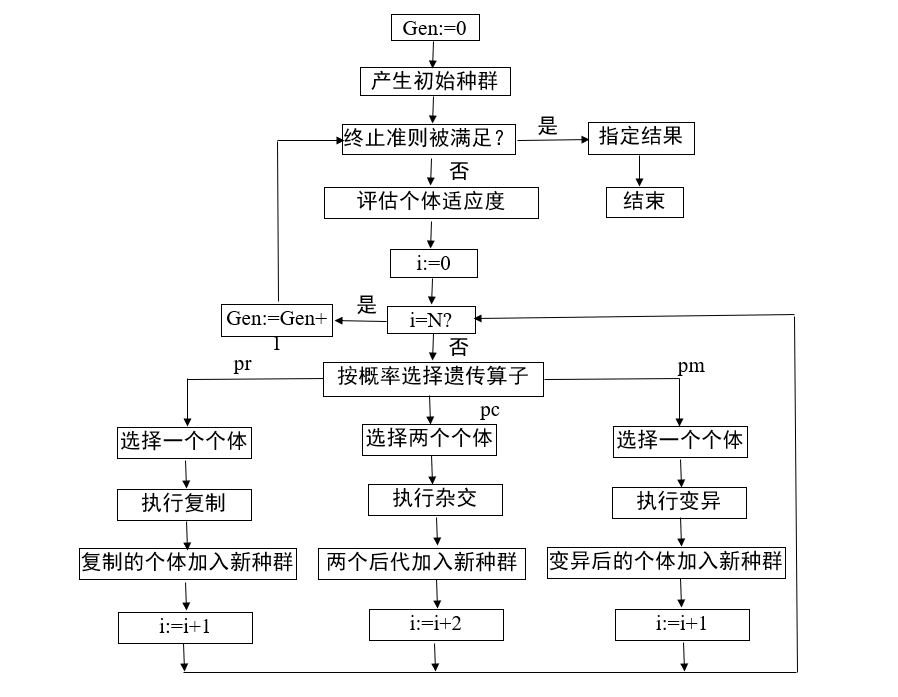
\includegraphics[scale=0.4]{images/GP_framework.png}
 		\caption{遗传程序设计的流程图}
 		\label{fig:label}
 	\end{figure}

\subsection{关键}
遗传程序设计所需解决的关键问题:	

(1)程序的表示;

(2)程序好坏的评价标准;

(3)遗传算子的设计。

\subsubsection{程序的表示}
在遗传程序设计中,种群中的个体是计算机程序。为了程序表示的简单性和容易验证程序的句法,遗传程序设计用LISP语言来表示程序。	

考虑一个简单的LISP程序,该程序简单地返回一个自然数n的平方:

>(defun square(n)(*nn))

SQUARE

下面是一个计算实数绝对值的LISP程序:

>(defun abs(x)(if(< x 0)(-x)(x)))

ABS

LISP程序的主体由类似于(*nn)和(if(< x 0)(-x)(x))的一些S-表达式所组成。

一般来说一个表示LISP程序的S-表达式通常由一些函数和端点组成。

构造LISP程序的S-表达式是以前缀表达式形式表示的。给定一个S-表达式,我们容易构造出它的语法树,而对该树进行先序遍历便可得到给定的S-表达式。

例如S-表达式(+12(if(> x 10)56))所对应的语法树如下图所示:
\begin{figure}[ht]
	\centering	
	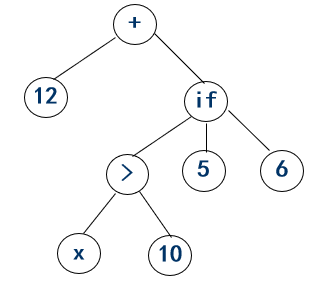
\includegraphics[scale=0.3]{images/syntactic_tree.png}
	\caption{S-表达式的语法树}
	\label{fig:label}
\end{figure}

\newpage
在语法树中,树的外部结点(叶结点)分别用变量x和常量5,6,10,12来标记,这些变量和常量通常称为端点,而内部结点分别用函数+,>,IF来标记。

\subsubsection{实现}
用遗传程序设计求解问题有以下五个基本步骤:
\begin{itemize}		
	\item 选择端点集;
	\item 选择函数集;
	\item 确定适应函数;
	\item 确定控制参数;
	\item 确定指定结果的方法和终止程序运行的条件。
\end{itemize}

\subsubsection{选择端点集和函数集}	
	在遗传程序设计中,计算机程序用LISP程序的语法树来表示。每一棵语法树的内部结点由一些函数构成,而叶结点由一些变量和常数构成。
	
	对于一个给定的问题,首先要确定由所有可能求解该问题的程序所组成的程序空间S。由于LISP程序通常可以由一些简单的函数、变量和常数经过有限次运算和复合而生成。因此若要指定程序空间S,我们只要指定可以构成中程序的函数集和端点集。
	
	函数集可以包含:
	
	(1)算数运算 +,-,*,/等;
	
	(2)数学函数 sin,cos,exp,log等;
	
	(3)布尔运算 AND,OR,NOT等;
	
	(4)条件运算 IF-THEN-ELSE等;
	
	(5)循环运算 DO-UNTIL,FOR,WHILE等。
	
	端点集通常由变量和常量组成。
	
\subsubsection{初始化}
	\begin{itemize}		
		\item 假设问题的端点集和函数集分别为T和F。
		\item 初始种群中的每个S-表达式,即每棵树,可按以下步骤产生:
		
		(1)首先建立一个根结点,从函数集F中随机地选择一个函数作为根结点的标记;
		
		(2)每当树中的一个结点被标记为函数集F中的一个函数$f$后,则为该结点建立$z(f)$个儿子结点,而每个儿子结点的标记从$C=F \bigcup T$中随机地选取;
		
		(3)每当树中一个结点被标记为端点集T中的一个元素时,则该结点成为树的一个叶结点;
		
		(4)如此反复进行,直到所有结点都被标记。
		\item 假定F=\{+,-,*,/\},T=\{a,b,c,d\}。下面给出了建立一棵树结构的过程:
			\begin{figure}[ht]
				\centering	
				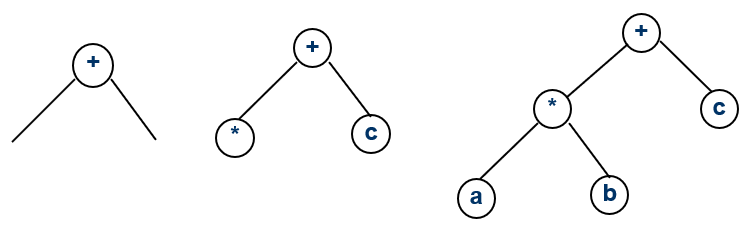
\includegraphics[scale=0.3]{images/build_tree.png}
				\caption{语法树的构建}
				\label{fig:label}
			\end{figure}
		\item 上述树生成过程可以有几种不同的实现方式:
		\item 确定适应函数:	
		\item 确定控制参数;
		\item 确定指定结果的方法和终止程序运行的条件。
		
		(1)完全法:该方法预先定义所要生成的树的最大深度Di,当要生成的结点的深度小于最大深度时,则从函数集F中随机地选取一个元素作为该结点的标记,当要生成的结点的深度等于最大深度时,则从端点集T中随机地选取一个元素作为该结点的标记。
		
		(2)生长法:该方法预先定义所要生成的树的最大深度Di,当要生成的结点的深度小于最大深度时,则从    中随机地选取一个元素作为该结点的标记,当要生成的结点的深度等于最大深度时,则从端点集T中随机地选取一个元素作为该结点的标记。
	
		(3)混合法:该方法预先定义所要生成的树的最大深度Di,对从2至最大深度的每一个深度,生成相同个数的树。对每一个深度,其中一半的树用完全法生成,而另一半用生成方法生成。
		
		例如,假定树的最大深度定义为6,种群中个体的个数为100,则用混合方法将分别产生深度为2,3,4,5,6的树各20个,其中深度为的树有10个用完全法产生,有10个用生成方法产生。
	\end{itemize}

\subsubsection{适应函数}
	适应性函数是遗传算法和遗传程序设计得以实现的关键因素,是评价个体好坏的定量表述,决定着演化过程中群体选择复制及群体整体性的质量。
	
	与其它演化算法相同,在遗传程序设计中,个体的适应性函数值是判断个体的质量的唯一办法。
	
	个体适应性函数值的计算方法是问题相关的,有多种方式度量个体的适应性函数值,有些方法是明确的,有些方法是隐含的。
	
	例如,若个体是下列程序:
	\begin{figure}[ht]
		\centering	
		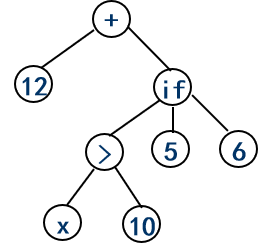
\includegraphics[scale=0.3]{images/program.png}
		\caption{程序示例}
		\label{fig:label}
	\end{figure}

	评估该程序好坏的一种方法是:
	
	(1)建立一个样本集$\{(x_{i},y_{i})|i=1,2,\Lambda,s\}$,其中$y_{i}$是当变量x取值为$x_{i}$时的期望输出;
	
	(2) 当$x=x_{i}(i=1,2,\Lambda,s)$时,运行该程序得到输出$z_{i}$;
	
	(3) 计算所得到的输出与期望输出之间的误差的绝对值之和$e=\Sigma|z_{i}-y_{i}|$;
	
	(4) 最后,用e作为该个体的适应性函数值。显然,适应性函数值越小,个体越好。
	
	若个体是判定树,则判定树的分类准确率可以作为个体的适应性函数值。若个体是游戏策略,则游戏策略与其它策略对奕时取胜的次数可以作为个体的适应性函数值。
	
	个体适应性函数值有以下几种形式:
	
	(1) 原始适应性函数值;
	
	原始适应性函数值是以问题本身的自然术语叙述的适应性函数值度量。
	
	(2) 标准适应性函数值;
	
	标准适应性函数值对原始适应性函数值作简单变换,使得标准适应性函数值越小,个体越好。
	
	(3) 调整适应性函数值;
	
	调整适应性函数值$\epsilon(0,1]$。调整适应性函数值越大,个体越好。
	
	(4) 正规化适应性函数值。
	
	正规化适应性函数值$\epsilon[0,1]$,在基于适应性函数值比例的选择策略中可直接用作选择概率。
	
	设计适应性函数,一般有以下几个步骤:
	
	(1) 原始适应性函数;
	
	按照目标函数的计算方法直接计算原始适应性函数值。
	
	(2) 标准化适应性函数;
	
	将得出的原始适应性函数表述为标准适应性函数。
	
	(3) 优化调整适应性函数;
	
	调整最优个体与次优个体的微小差别。
	
	(4) 正规化适应性函数。
	
	正规化(归一化)已优化调整的适应性函数值。
	
\subsection{父体选择策略}		
	(1) 通常,遗传程序设计使用基于适应性函数值比例的选择策略。
	
	(2) 若种群规模在1000以上,则经常使用一种贪婪过度选择策略。
	
	(3)该策略首先将种群中的个体按适应性函数值排序,然后将种群中的个体分为两部分。第一部分包含种群$x\%$的最好个体,另一部分包含其它$(1-x\%)$的个体。当进行父体选择时,80\%的选择在第一部分中进行,20\%的选择在第二部分中进行。x的取值以来于种群规模,通常通过实验确定。
	\begin{figure}[ht]
		\centering	
		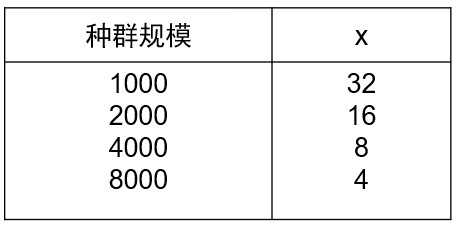
\includegraphics[scale=0.3]{images/x_value.png}
		\caption{x的取值}
		\label{fig:label}
	\end{figure}
	
	从上图可以看出,随着种群规模的增加,x不断减小,选择压力逐步增大。
	
\subsection{遗传算子}
	遗传程序设计中的遗传算子主要有复制、杂交和变异。变异算子的作用不及遗传算法中重要。
	
	(1) 复制
	
	复制算子首先按照某种基于适应性函数值比例的选择策略从种群中选择一个个体,然后将该个体不加改变地复制到下一代种群。
	
	复制算子有一个参数$p_{r}$,通常取$p_{r}=0.1$。
	
	(2) 杂交
	
	杂交算子分别从两个父体中随机地选择一个杂交点,然后交换父体中以杂交点为根结点的子树产生两个后代。
	\begin{figure}[ht]
		\centering	
		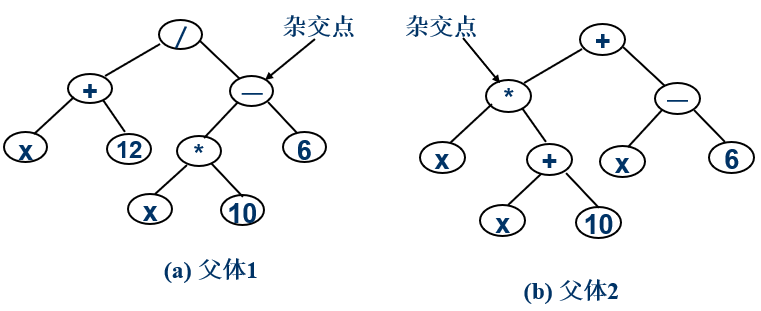
\includegraphics[scale=0.25]{images/Hybridization1.png}
		\caption{杂交前}
		\label{fig:label}
	\end{figure}	
	\begin{figure}[ht]
		\centering	
		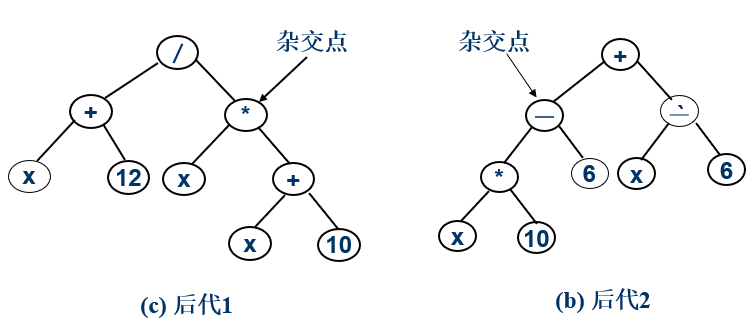
\includegraphics[scale=0.25]{images/Hybridization2.png}
		\caption{杂交后}
		\label{fig:label}
	\end{figure}

	 杂交算子有两个参数 $p_{c}$和$p_{cn}$,$p_{c}$是按概率选择遗传算子时选择杂交算子的概率,而$p_{cn}$是在进行杂交时,在父体中选择内结点作为杂交点的概率。通常取$p_{c}=0.9$和$p_{cn}=0.9$。
	
	在对父体进行杂交后,后代树的深度有可能加大。为了有效地利用计算机资源,防止产生巨型个体,遗传程序设计通常设置一个最大允许深度$D_{c}$进行控制。
	
	若杂交后,有一个后代的深度超过了最大允许深度,则随机地选取一个父体代替该后代;若两个后代的深度都超过了最大允许深度,则用两个父体代替这两个后代。
	
	(3) 变异
	
	\parindent=19pt
	变异算子首先在父体中随机地选择一个结点,然后删除以该结点为根结点的子树,并在该结点处插入一个随机生成的子树。
	\begin{figure}[ht]
		\centering	
		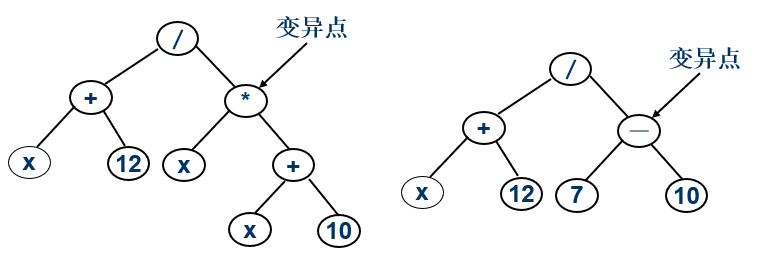
\includegraphics[scale=0.25]{images/variation.png}
		\caption{变异}
		\label{fig:label}
	\end{figure}
	
	变异算子有两个参数$p_{m}$和$p_{mm}$。$p_{m}$是按概率选择遗传算子时选择变异算子的概率,而$p_{mm}$是在进行变异时,在父体中选择内结点的概率。
	
	值得注意的是J.R.Koza建议$p_{m}$,也就是说在遗传程序设计中不使用变异算子。近年来的遗传程序设计实践建议使用变异算子,但是以较低的概率。

\section{简单实例}
\subsection{简单符号回归}
问题:给定20个样本点$(x_{1},y_{1}),(x_{1},y_{1}),\Lambda,(x_{20},y_{20})$,其中$x_{i}(i=1,2,\Lambda,20)$是区间[-1,1]中的随机数,而$y_{i}=x_{i}^{4}+x_{i}^{3}+x_{i}^{2}+x_{i}$,求出拟合这些样本点的函数。

  求解该问题的遗传程序设计如下:

  (1)端点集

  端点集可取为$T=\{X\}$。

  (2)函数集

  函数集可仅由算术运算加法和乘法组成。一个更一般的选择是$F=\{+,-,*,/,sin,cos,exp,ln\}$。

  (3)适应值度量

  个体$f$的原始适应值用下式计算:$err(f)=\Sigma|f(x_{i})-y_{i}|$。

  (4)父体选择策略

  使用轮盘赌选择。

  (5)种群初始化和算法终止准则

  用混合法产生初始种群。而当$|f(x_{i})-y_{i}|<0.01(i=1,2,\Lambda,n)$或算法运行到预先指定的最大演化代数时,终止算法运行。

  (6)参数设置
	\begin{figure}[ht]
		\centering	
		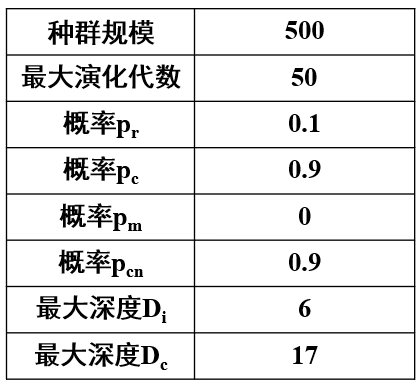
\includegraphics[scale=0.5]{images/parameter.png}
		\caption{参数设置}
		\label{fig:label}
	\end{figure}

  \newpage
  求解结果如下图所示:
 	\begin{figure}[ht]
  		\centering	
  		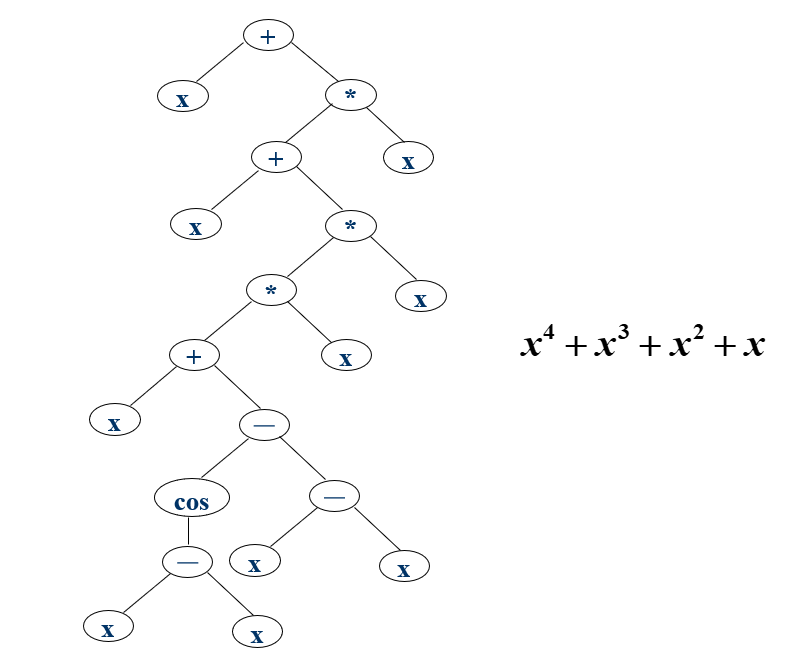
\includegraphics[scale=0.5]{images/answer4.png}
  		\caption{求解结果}
  		\label{fig:label}
  	\end{figure}
\subsection{求解数学恒等式}
求解数学恒等式涉及发现一个新的且不明显的数学表达式,使得该表达式与给定的表达式在某个定义域内恒等。

问题:给定数学表达式$cos(2x)$,我们希望发现与$cos(2x)$恒等的数学表达式。

将该问题视为一个符号回归问题。通过在某个区间内抽取一个随机样本,并计算给定函数在该样本的函数值,这样形成一组样本点,对所形成的样本点作符号回归。

由于$cos(2x)$是一个三角函数,所以在区间$[0,2\pi]$内随机地抽取20个值。利用这20个样本点$(x_{1},y_{1}),(x_{1},y_{1}),\Lambda,(x_{20},y_{20})$进行符号回归。

求解该问题的遗传程序设计如下:

(1)端点集

$T=\{X,1.0\}$

(2)函数集

$F=\{+,-,*,/,sin\}$

(3) 适应值度量

个体f的原始适应值用下式计算:$err(f)=\Sigma|f(x_{i})-y_{i}|$

(4)父体选择策略

使用轮盘赌选择。

(5)种群初始化和算法终止准则

用混合法产生初始种群。而当$|f(x_{i})-y_{i}|<0.01(i=1,2,\Lambda,n)$或算法运行到预先指定的最大演化代数时,终止算法运行。

\newpage
(6)参数设置
    \begin{figure}[ht]
    	\centering	
	   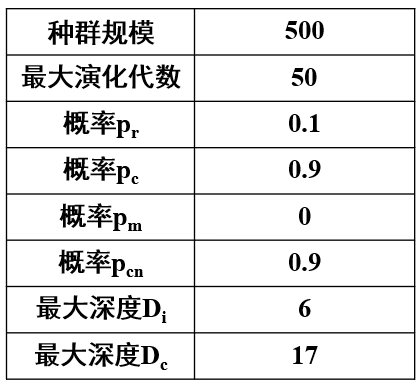
\includegraphics[scale=0.45]{images/parameter.png}   
	   \caption{参数设置}
	   \label{fig:label}
    \end{figure}

求解结果如下图所示:	
	\begin{figure}[ht]
	\centering	
	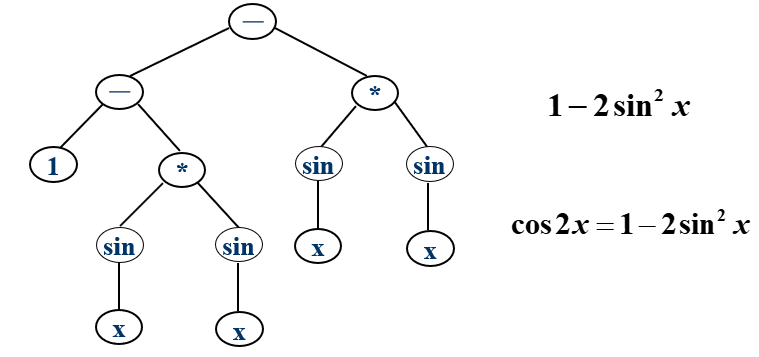
\includegraphics[scale=0.45]{images/A1.png}
	\caption{求解结果1}
	\label{fig:label}
	\end{figure}
	\begin{figure}[ht]
		\centering	
		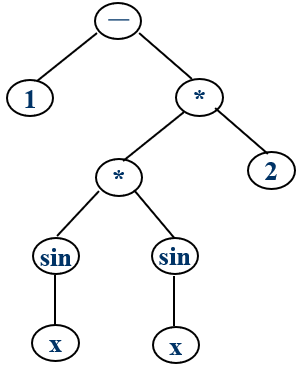
\includegraphics[scale=0.45]{images/A2.png}
		\caption{求解结果2}
		\label{fig:label}
	\end{figure}
	\begin{figure}[ht]
		\centering	
		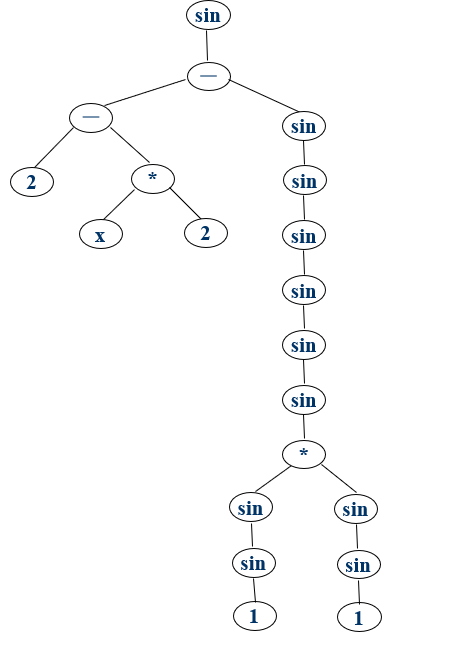
\includegraphics[scale=0.45]{images/A3.png}
		\caption{求解结果3}
		\label{fig:label}
	\end{figure}
\newpage
\section{应用领域}
遗传程序设计的应用领域很广,作为一种不需要先验性假设的寻找问题解的有效途径,其在以下几个领域中都得到了广泛的应用:

(1)预测和分类:使用历史数据库来预测新事例。

(2)符号压缩:发现各变量间的隐含关系。

(3)机器人:控制机器人行为,使其对环境做出反应。

(4)人工生命:用计算机模拟生物的自然进化或发现规律。

(5)神经网络设计“设计神经网络结构、发现学习规则和相关权值,以使神经网络完成指定的任务。

(6)图像和信号处理:图像识别、图像恢复、图像和声音的压缩等。

(7)多Agent系统的自动设计:多个Agent协作共同处理实际问题。

(8)游戏策略:发现一个策略打败对手。

(9)艺术:声音、三维图像的生成、计算机动画等。

\newpage
\section{实际应用}
近年来,许多学者对短期电价预测进行了大量的研究,出现各式各样的电价预测方法,其中主要有时间序列法、神经网络、支持向量机等智能方法,但都有其缺点。时间序列法对数据要求较高,无法考虑负荷等其他因素的影响,用线性模型表达电价的非线性关系有一定的局限性;神经网络容易陷入局部极小值和过拟合的现象;支持向量机的推广能力差。遗传程序设计无需事先人为给定数学模型,它能够根据与问题有关的终结点集和函数集,在进化的过程中动态地生成与历史数据相拟合的数学模型,从而可以预测出电价的未来趋势。本节将介绍遗传程序设计在短期电价预测中的应用,通过和时间序列法的预测结果进行比较,验证其在短期电价预测中的可行性和有效性。

\subsection{短期电价预测的遗传程序设计方法}
将历史电价数据和负荷数据作为输入数据,在预测之前先把数据分为训练数据和预测数据,分别用于建模和预测。由于日前市场中24时点电价差异较大,单一模型很难全面反映不同时点的电价特点,因此考虑建立24个不同的模型对24点日前电价分别进行预测。

具体实现步骤如下:

(1)数据预处理。如果资料的收集和选择不好,就会直接影响预测的质量,所以要对收集的资料进行预处理。

(2) GP预测电价建模。为找到最优的短期电价预测模型,选择合适的参数非常重要,经过多次测试后选取的参数如下:
	\begin{figure}[ht]
		\centering	
		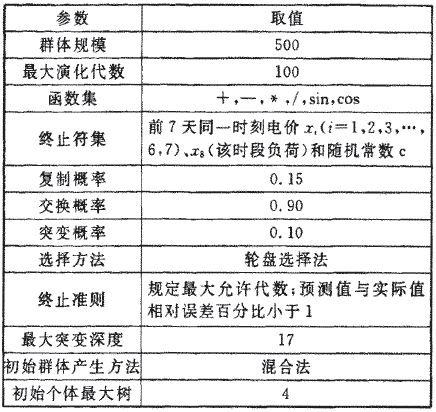
\includegraphics[scale=0.6]{images/example_parameter.png}
		\caption{GP演化建模参数}
		\label{fig:label}
	\end{figure}

\newpage
(3)寻找最优预测模型。将选取的样本数据集作为GP演化建模的训练样本集,寻找出最优的短期电价预测模型,利用最优模型对日电价进行预测。

具体工作流程如下图所示(图中Gen代表遗传代数):
	\begin{figure}[ht]
		\centering	
		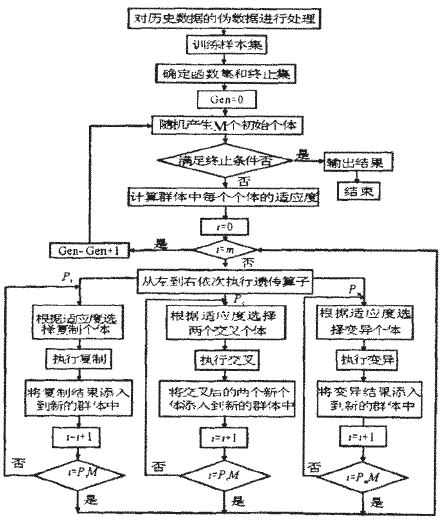
\includegraphics[scale=0.6]{images/example_workflow.png}
		\caption{GP短期电价预测流程图}
		\label{fig:label}
	\end{figure}

\subsection{算例分析}
运用所建模型,采用美国加利福利亚州电力市场1999年3月1日-3月17日的历史电价数据,对3月18日的24个时段的电价进行预测。为了对比分析,分别给出了用时间序列法(ARIMA)和遗传程序设计(GP)的预测结果,其实际值、预测值如图17所示:
	\begin{figure}[ht]
		\centering	
		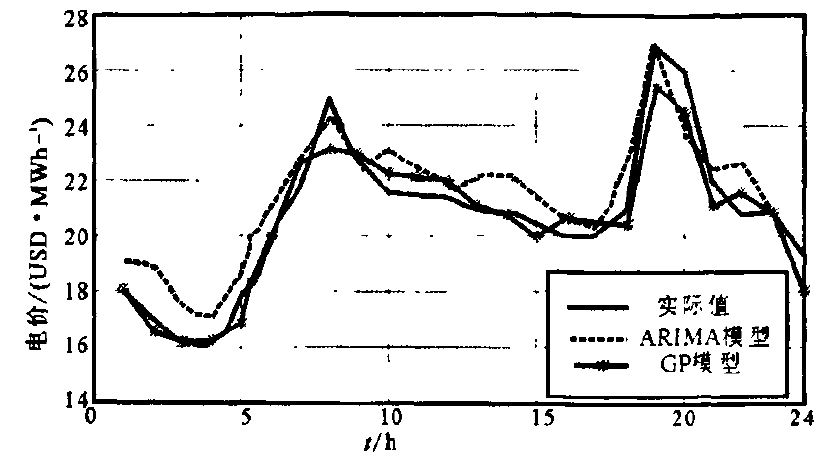
\includegraphics[scale=0.6]{images/example_result_fig.png}
		\caption{GP模型与ARIMA模型的预测结果对比图}
		\label{fig:label}
	\end{figure}

\newpage
图18逐点列出了实际电价、ARIMA预测和GP预测的结果:
	\begin{figure}[ht]
		\centering	
		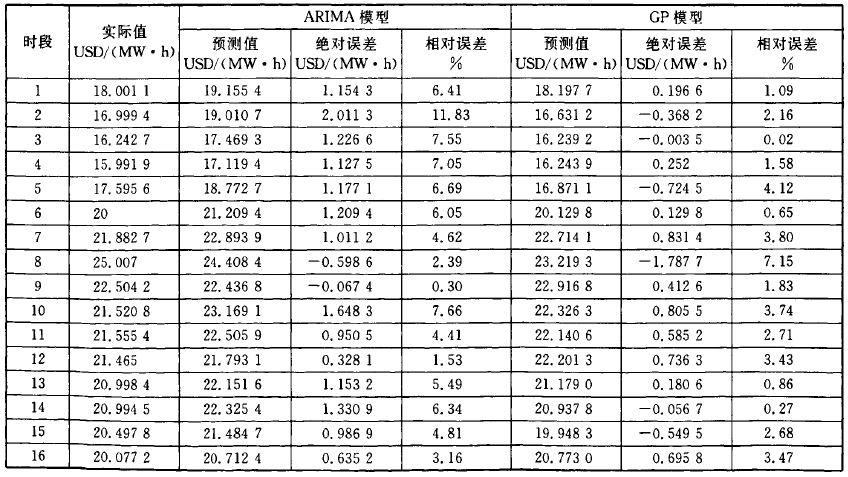
\includegraphics[scale=0.6]{images/example_result_table.png}
		\caption{1999年3月18日24个时段的电价预测结果图}
		\label{fig:label}
	\end{figure}

由图18可以看出,GP的预测精度明显好于ARIMA预测的精度,平均相对误差明显减小,其中用ARIMA模型预测的平均相对误差为5.17%,用GP模型预测的平均相对误差为2.86%。结果表明,用GP预测方法所得的结果令人满意。

\subsection{结论}
本节本文提出了一种基于遗传程序设计的短期电价预测方法,该方法所需数据较少,很大程度上提高了拟合的精度,尤其是数据量比较少或者对数据的性态不太了解时,利用GP方法来发现数据间的关系是一种比较简单且可行的方法,并且终结点集中的随机常数c能够有效的平衡与电价有关的影响,由曲线拟合情况和与时间序列法预测的比较结果可以看出,该方法在短期电价预测中是有效可行的。

\section{未来展望}
作为演化计算最新的分支,遗传程序设计所面临的更为复杂而具有挑战性的课题,是实现计算机程序设计的自动化。解决这个难题需要演化计算、软件工程、最优化、系统科学、人工智能和应用数学等许多领域的共同努力。相信在不久的将来,遗传程序设计会对计算机自动程序设计的发展起到很大的作用。

\newpage
\section{参考文献}
[1] Koza J R. Genetic Programming:On the Programming of Computers by Means of Natural Selection. Cambridge,MA:MIT Press,1992.

[2] Chi Zhou,gene expression programming and rule induction for domain knowledge discovery and management,Doctoral dissertation,Department of Computer Science,University of Illinois at Chicago,Chicago,IL,2003.

[3] Clack C,Yu T . Performance enhanced genetic programming. In:Proc of the 6th Conf on Evolutionary Programming,Lecture Notes in Computer Science 1213 . Indianapolis,Indiana,USA,1997.

[4] Holland J H Scientific American,1992-4l4.

[5] Koza J R.Genetic Programming1 On the Programming of Computers by Means D,"Nagural Selection.Cambridgel MIT Press,1992.

[6] 潘正君,康立山,陈毓屏.演化计算[M] 北京:清华大学出版社,1998.

[7] 张显,王锡凡.短期电价预测综述[J].电力系统自动化,2006,30(3):92-101.

[8] 周明.严正,倪以倍,等.含误差预测校正的ARIMA电价预测新方法[J].中国电机工程学报,2004,24(12):63-68.

[9] 刘勇、康立山、陈毓屏.非数值并行算法(第三册)——遗传算法. 北京:科学出版社,1995.

[10] 王小平,曹立明.遗传算法——理论,应用与软件实现[M].西安:西安交通大学出版社,2005.

\end{document}
